\section{Theoretical Background} \label{theory}

This chapter deals with the past and present research in the relevant area which include literature review. This includes 
the significance of precise modelling of the ship's speed and its subsequent use in forecasting the ship's operation.
The theoretical background of Random Forest Regression will be discussed in this chapter 

\subsection{Literature Review}

This section provides 

This section provides an overview on the scientific papers relating to this thesis. There have been considerable amount of research on machine learning approach to predict ship Fuel Oil Consumption (FOC). Gkerekos \cite{Gkerekos.2019} and Abebe \cite{Abebe.2020} compares the performance of different machine learning methods to predict FOC. Besicki \cite{BalBesikci.2016} used Artificial Neural Network (ANN) to predict FOC. These papers demonstrate the capability of machine learning method to predict vessel's FOC with different scores and errors in their respective model. Worth noting that each of these scientific papers used different type of data and data source to make their prediction. Gkerekos \cite{Gkerekos.2019} use both the noon- and AIS data from ???. Besicki \cite{BalBesikci.2016} exclusively use noon data from ?? while \cite{Abebe.2020} performs fusion on both the noon- and AIS data from ??

Findings from Gkerekos \cite{Gkerekos.2019}, Li \cite{Li.2022} and \cite{Abebe.2020} shows that Random Forest model is able to make better prediction compared simpler machine learning model such as linear regression. 

The findings from this paper shows the ability of machine learning method to make accurate prediction of the vessel's FOC. This paper also conclude that using automatic data logger sensor based data could potentially increase the model performance. 
\subsection{Random Forest Regression (RFR)}


\begin{figure}[h]
\centering
\begin{minipage}[b]{.5\textwidth}
    \centering
    \begin{tikzpicture}[x=0.75pt,y=0.75pt,yscale=-1,xscale=1]
    %uncomment if require: \path (0,433); %set diagram left start at 0, and has height of 433
    
    %Shape: Square [id:dp5731268858272198] 
    \draw   (180,110) -- (370,110) -- (370,300) -- (180,300) -- cycle ;
    %Straight Lines [id:da615072570759449] 
    \draw    (250,110) -- (250,300) ;
    %Straight Lines [id:da8002566967918264] 
    \draw    (300,110) -- (300,300) ;
    %Straight Lines [id:da4409034763483005] 
    \draw    (180,230) -- (250,230) ;
    %Straight Lines [id:da07514682530914596] 
    \draw    (300,170) -- (370,170) ;
    
    % Text Node
    \draw (131,192.4) node [anchor=north west][inner sep=0.75pt]    {$X_{2}$};
    % Text Node
    \draw (261,340.4) node [anchor=north west][inner sep=0.75pt]    {$X_{1}$};
    % Text Node
    \draw (157,222.4) node [anchor=north west][inner sep=0.75pt]    {$t_{2}$};
    % Text Node
    \draw (201,252.4) node [anchor=north west][inner sep=0.75pt]    {$R_{1}$};
    % Text Node
    \draw (201,162.4) node [anchor=north west][inner sep=0.75pt]    {$R_{2}$};
    % Text Node
    \draw (268,192.4) node [anchor=north west][inner sep=0.75pt]    {$R_{3}$};
    % Text Node
    \draw (321,132.4) node [anchor=north west][inner sep=0.75pt]    {$R_{4}$};
    % Text Node
    \draw (321,220.4) node [anchor=north west][inner sep=0.75pt]    {$R_{5}$};
    % Text Node
    \draw (241,310.4) node [anchor=north west][inner sep=0.75pt]    {$t_{1}$};
    % Text Node
    \draw (291,312.4) node [anchor=north west][inner sep=0.75pt]    {$t_{3}$};
    % Text Node
    \draw (381,162.4) node [anchor=north west][inner sep=0.75pt]    {$t_{4}$};
    
    \end{tikzpicture}
    
    \captionof{figure}{Example of partition space} 
    \label{fig:partitionspace}
\end{minipage}%
\begin{minipage}[b]{.5\textwidth}
    \centering
    \begin{tikzpicture}
        \tikzset{level distance=65pt,sibling distance=10pt,edge from parent/.style=
        {draw,edge from parent path={(\tikzparentnode.south)
                                -- +(0,-8pt)
                                -| (\tikzchildnode)}}}
    \Tree [.$X_1\leq t_1$ [.$X_2\leq t_2$ [.$R_1$ ] [.$R_2$ ] ]
        [.$X_1\leq t_3$ [.$R_3$ ]
        [.$X_2\leq t_4$ [.$R_4$ ] [.$R_5$ ] ] ] ]
    \end{tikzpicture}
    \captionof{figure}{Example of partition tree} 
    \label{fig:partitiontree}
\end{minipage}
\end{figure}


\begin{tikzpicture}[x=0.75pt,y=0.75pt,yscale=-1,xscale=1]
    %uncomment if require: \path (0,452); %set diagram left start at 0, and has height of 452
    
    %Shape: Axis 2D [id:dp697661158302031] 
    \draw  (220,297.8) -- (517.5,297.8)(249.75,80) -- (249.75,322) (510.5,292.8) -- (517.5,297.8) -- (510.5,302.8) (244.75,87) -- (249.75,80) -- (254.75,87)  ;
    %Image [id:dp23308396965327827] 
    \draw (245,305) node [rotate=-40.58] {
\includegraphics[width=26.87pt,height=72.39pt]{02_figures/ferry.jpg}};
    
    
    
    
\end{tikzpicture}

Suppose the following decision tree regressor


\subsection{Ship speed}


\subsection{Modelling}




